\documentclass[12pt]{beamer}
\usepackage{pgf}
\usepackage[danish]{babel}
\usepackage[utf8]{inputenc}
\usepackage{beamerthemesplit}
\usepackage{graphics,epsfig, subfigure}
\usepackage{url}
\usepackage{srcltx}
\usepackage{hyperref}

\usepackage{fancybox}
\usepackage{listings}
\lstset{
  language=C,                % choose the language of the code
   basicstyle=\footnotesize,        % the size of the fonts that are used for the code
    keywordstyle=\color{blue},       % keyword style
     commentstyle=\color[rgb]{0.13,0.54,0.13},
  numbers=left,                   % where to put the line-numbers
  stepnumber= 0.3,                   % the step between two line-numbers.        
  numbersep=1pt,                  % how far the line-numbers are from the code
  backgroundcolor=\color{white},  % choose the background color. You must add \usepackage{color}
  showspaces=false,               % show spaces adding particular underscores
  showstringspaces=false,         % underline spaces within strings
  showtabs=false,                 % show tabs within strings adding particular underscores
  tabsize=2,                      % sets default tabsize to 2 spaces
  captionpos=b,                   % sets the caption-position to bottom
  breaklines=true,                % sets automatic line breaking
  breakatwhitespace=true,         % sets if automatic breaks should only happen at whitespace
 % title=\lstname,                 % show the filename of files included with \lstinputlisting;
}
\definecolor{kugreen}{RGB}{50,93,61}
\definecolor{kugreenlys}{RGB}{132,158,139}
\definecolor{kugreenlyslys}{RGB}{173,190,177}
\definecolor{kugreenlyslyslys}{RGB}{214,223,216}
\setbeamercovered{transparent}
\mode<presentation>
\usetheme[numbers,totalnumber,compress,sidebarshades]{PaloAlto}
\setbeamertemplate{footline}[frame number]

  \usecolortheme[named=kugreen]{structure}
  \useinnertheme{circles}
  \usefonttheme[onlymath]{serif}
  \setbeamercovered{transparent}
  \setbeamertemplate{blocks}[rounded][shadow=true]

\logo{
\includegraphics[width=0.8cm]{fga_logo.png}}
%\useoutertheme{infolines} 
\title{Métodos de Desenvolvimento de Software - Ciclo de Vida}

\author{Dra. Carla Rocha}
\institute{Engenharia de Software \\ Universidade de Brasília}
\date{}
\begin{document}
\frame{\titlepage \vspace{-0.5cm}
}
\frame
{
\frametitle{Agenda}
\tableofcontents%[pausesection]
}
  
\section{Crise de Software}
\begin{frame}
 \frametitle{Crise de Software}
 \begin{itemize}
  \item Termo utilizado nos anos 1970
  %\pause
  \item Expressava as dificuldades do desenvolvimento de software frente ao
  \begin{itemize}
   \item rápido crescimento da demanda por software
   %\pause
   \item   complexidade dos problemas a serem resolvidos
   %\pause
   \item  inexistência de técnicas estabelecidas para o desenvolvimento de sistemas que funcionassem adequadamente
  \end{itemize}
 \end{itemize}
\end{frame}


\begin{frame}[fragile]
 \frametitle{Crise de Software \\ Exemplo - Código Quake III Arena}
 \begin{itemize}
  \item Implementação da raiz quadrada inversa
 \end{itemize}
 \begin{lstlisting}
float Q_rsqrt( float number)
{
  int i;
  float x2, y;
  const float threehalfs = 1.5F;
  x2 = number * 0.5F;
  y = number;
  i = * ( int * ) &y; // evil floating point bit level hacking
  i = 0x5f3759df - ( i >> 1 ); // what the f***?
  y = * ( float * ) &i;
  y = y * ( threehalfs - ( x2 * y * y ) ); // 1st iteration
  return y;
}  
 \end{lstlisting}
\end{frame}

\begin{frame}
\frametitle{Resposta à Crise de Software}
\begin{block}{Processo de Software}
 Abordagem sistemática, disciplinada e possível de
ser medida para o desenvolvimento, operação e manutenção do software
\end{block}
\end{frame}



\begin{frame}
 \frametitle{Processo de Software}
 \begin{block}{}
  Consiste em uma série de atividades, práticas, eventos, ferramentas e
métodos que garantem, técnica e administrativamente que o software
pode ser desenvolvido com qualidade e de maneira \textbf{organizada, disciplinada
e previsível}
 \end{block}
\end{frame}


\begin{frame}
 \frametitle{Processo de Software}
\frametitle{Fases do Processo de Software}
\begin{figure}
 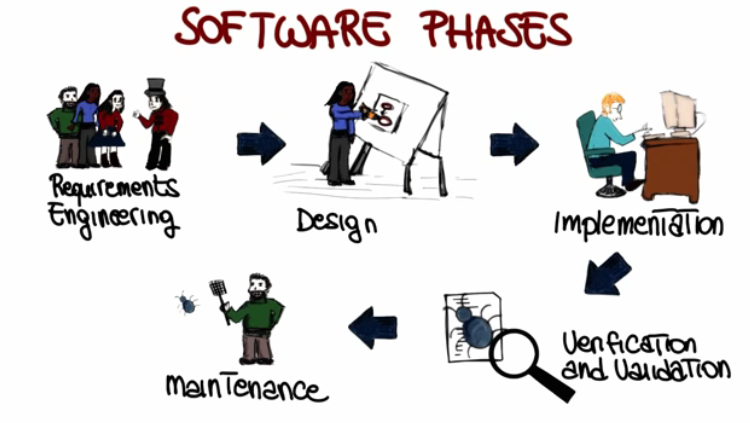
\includegraphics[width = \textwidth]{figs/fig20.png}
\end{figure}
\end{frame}

\begin{frame}
 \frametitle{Requisitos}
 \begin{block}{}
   É o processo para estabelecer quais são as necessidades dos \textit{stakeholders} que devem ser solucionados pelo software
 \end{block}
 \begin{figure}
 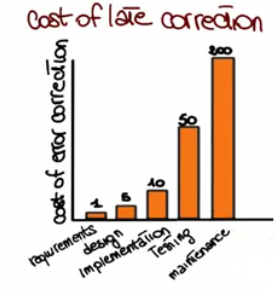
\includegraphics[width = 0.5\textwidth]{figs/fig22.png}
\end{figure}
\end{frame}

\begin{frame}
 \frametitle{Projeto (Design)}
\begin{itemize}
 \item Atividades de projeto:
 \begin{itemize}
  \item Projeto da Arquitetura
  \item Especificação abstrata
  \item Projeto de Interface
  \item Projeto do Componente
  \item Estrutura de dados
  \item Projeto de Arquitetura
 \end{itemize}
\end{itemize}

\end{frame}


\begin{frame}
 \frametitle{Projeto (Design)}
\begin{itemize}
 \item Produtos do Projeto:
 \begin{itemize}
  \item Estrutura do Sistema
  \item Especificação de software
  \item Especificação de Interface
  \item Especificação do Componente
  \item Especificação da Estrutura de dados
  \item Especificação do Algoritmo
 \end{itemize}
\end{itemize}
\end{frame}

\begin{frame}
 \frametitle{Implementação}
\begin{itemize}
 \item Quatro pilares:
 \begin{itemize}
  \item Redução da Complexidade
  \item Antecipar diversidade
  \item Estruturar para validação
  \item Uso de  padrões (interno/externo)
 \end{itemize}
\end{itemize} 
\end{frame}

\begin{frame}
 \frametitle{Verificação e Validação}
\begin{itemize}
 \item \textbf{Validação}:  construimos o sistema correto?
 \item \textbf{Verificação}: construimos o sistema corretamente?
\end{itemize} 
 \begin{figure}
 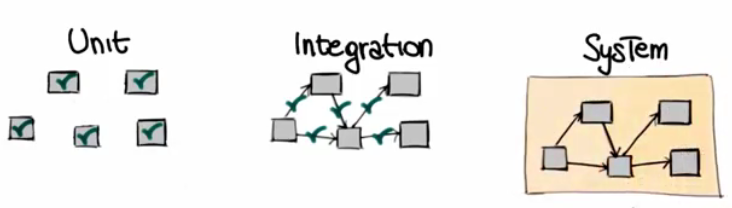
\includegraphics[width = 0.9\textwidth]{figs/fig23.png}
\end{figure}
\end{frame}

\begin{frame}
 \frametitle{Manutenção}

 \begin{figure}
 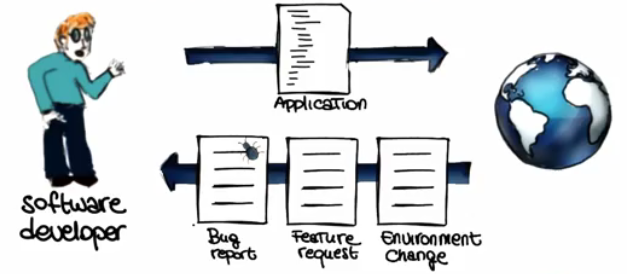
\includegraphics[width =\textwidth]{figs/fig24.png}
\end{figure}
\end{frame}

\begin{frame}
 \frametitle{Processo de Software}
 \begin{block}{Problema}
 Uma das \textbf{maiores dificuldades} encontradas pelas empresas
de software é o \textbf{gerenciamento} de seus \textbf{processos de software}
 \end{block}

 \begin{block}{Solução}
  \textbf{Modelos de Processo de Software}
 \end{block}
\end{frame}

\section{Modelo de Processo}
\begin{frame}
 \frametitle{Modelo de Processo}
 \begin{itemize}
  \item Escolhido de acordo com a natureza da aplicação e as características do projeto
  %\pause
\item Corresponde ao que usualmente se chama de Ciclo de Vida (ISO 9000/3)
%\pause
\item Há vários de modelos de processo de software propostos
 \end{itemize}
\end{frame}

\begin{frame}
 \frametitle{Modelo de Processo}
\begin{figure}
 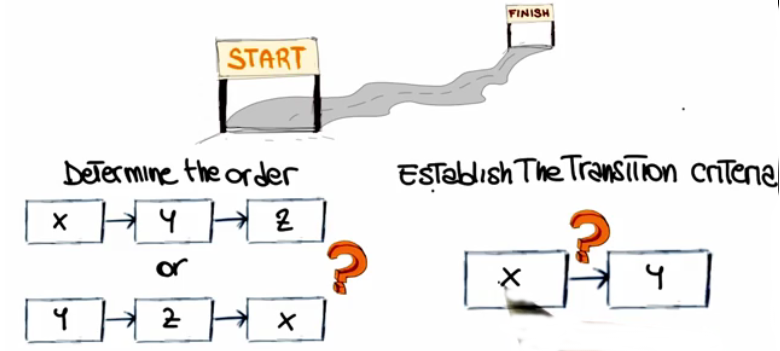
\includegraphics[width = \textwidth]{figs/fig21.png}
\end{figure}
\end{frame}


\begin{frame}
 \frametitle{Modelos de Processo de Software}
 \begin{itemize}
  \item  O Modelo Sequencial Linear
  \begin{itemize}
   \item também chamado Modelo Cascata ou Ciclo de Vida Classico
  \end{itemize}
  %\pause
  \item O Paradigma de Prototipação
  %\pause
  \item O Modelo RAD (Rapid Application Development)
  %\pause
  \item Modelos Evolutivos de Processo de Software
  \begin{itemize}
   \item O Modelo Incremental
   \item O Modelo Espiral
   \item O Modelo de Montagem de Componentes
  \end{itemize}
 \end{itemize}
\end{frame}


\begin{frame}
\frametitle{Modelos de Processo de Software}
 \begin{figure}
  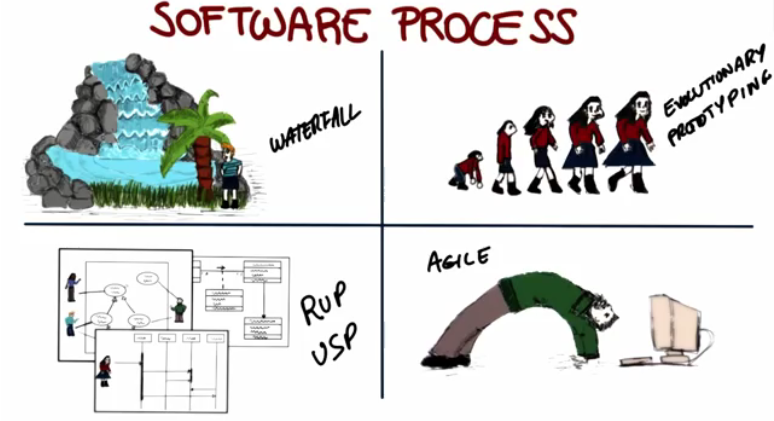
\includegraphics[width = \textwidth]{figs/fig19.png}
 \end{figure}
\end{frame}

\section{Bibliografia}

\begin{frame}
 \frametitle{Bibliografia Sugerida}
 \begin{itemize}
  \item "Construindo Software como Serviço (SaaS): Uma Abordagem Ágil Usando Computação em Nuvem" - Introdução

 \end{itemize}

\end{frame}
% 


\end{document}
